\jxhj{%教学后记
	}
\skrq{%授课日期
	2017年10月12日 4-5节}
\ktmq{%课题名称
	 刀具半径补偿的应用(二)}
\jxmb{%教学目标,每行前面要加 \item
	\item 掌握用刀补去残料。
	\item 掌握去材料刀补的计算;
	\item 掌握多个刀补的编程;
	\item 巩固粗/精加工刀补值的确定。
 }
\jxzd{%教学重点,每行前面要加 \item
	\item 用刀补去残料;
	\item 去材料刀补的计算。 }
\jxnd{%教学难点,每行前面要加 \item
	\item 去材料刀补的计算。 }
\jjff{%教学方法
	通过讲述、举例、演示法来说明;}

\makeshouye %制作教案首页

%%%%教学内容
\subsection{组织教学}
\begin{enumerate}[\hspace{2em}1、]
	\item 集中学生注意力;
	\item 清查学生人数;
	\item 维持课堂纪律;
\end{enumerate}
\subsection{复习导入及主要内容}
\begin{enumerate}[1、]
\item 刀补的概念
\item G40、G41/G42指令的使用;
\item 注意事项;
\item 刀补的编程;
\item 刀补值的计算。
\end{enumerate}



\subsection{教学内容及过程}

\subsubsection{去残料刀补的计算}
步骤

1、计算最大残料值

以实际毛坯尺寸来计算

2、根据刀具直径确定粗加工刀补值

刀具半径+单边余量(0.2-0.6)

3、根据刀具直径确定加工宽度

刀具直径的50\%-80\%

也可: (残料-粗加工刀补)/次数

4、刀补值的计算:

去残料刀补=粗加工刀补+加工宽度×次数

5、判断残料是否去完

最大刀补+刀具半径>最大残料  表示已去完

6、其他:

根据最大刀补确定切入切出半径

最大刀补不能大于最小内凹圆弧半径

\subsubsection{去残料刀补的计算}

\begin{figure}[h]
	\centering
	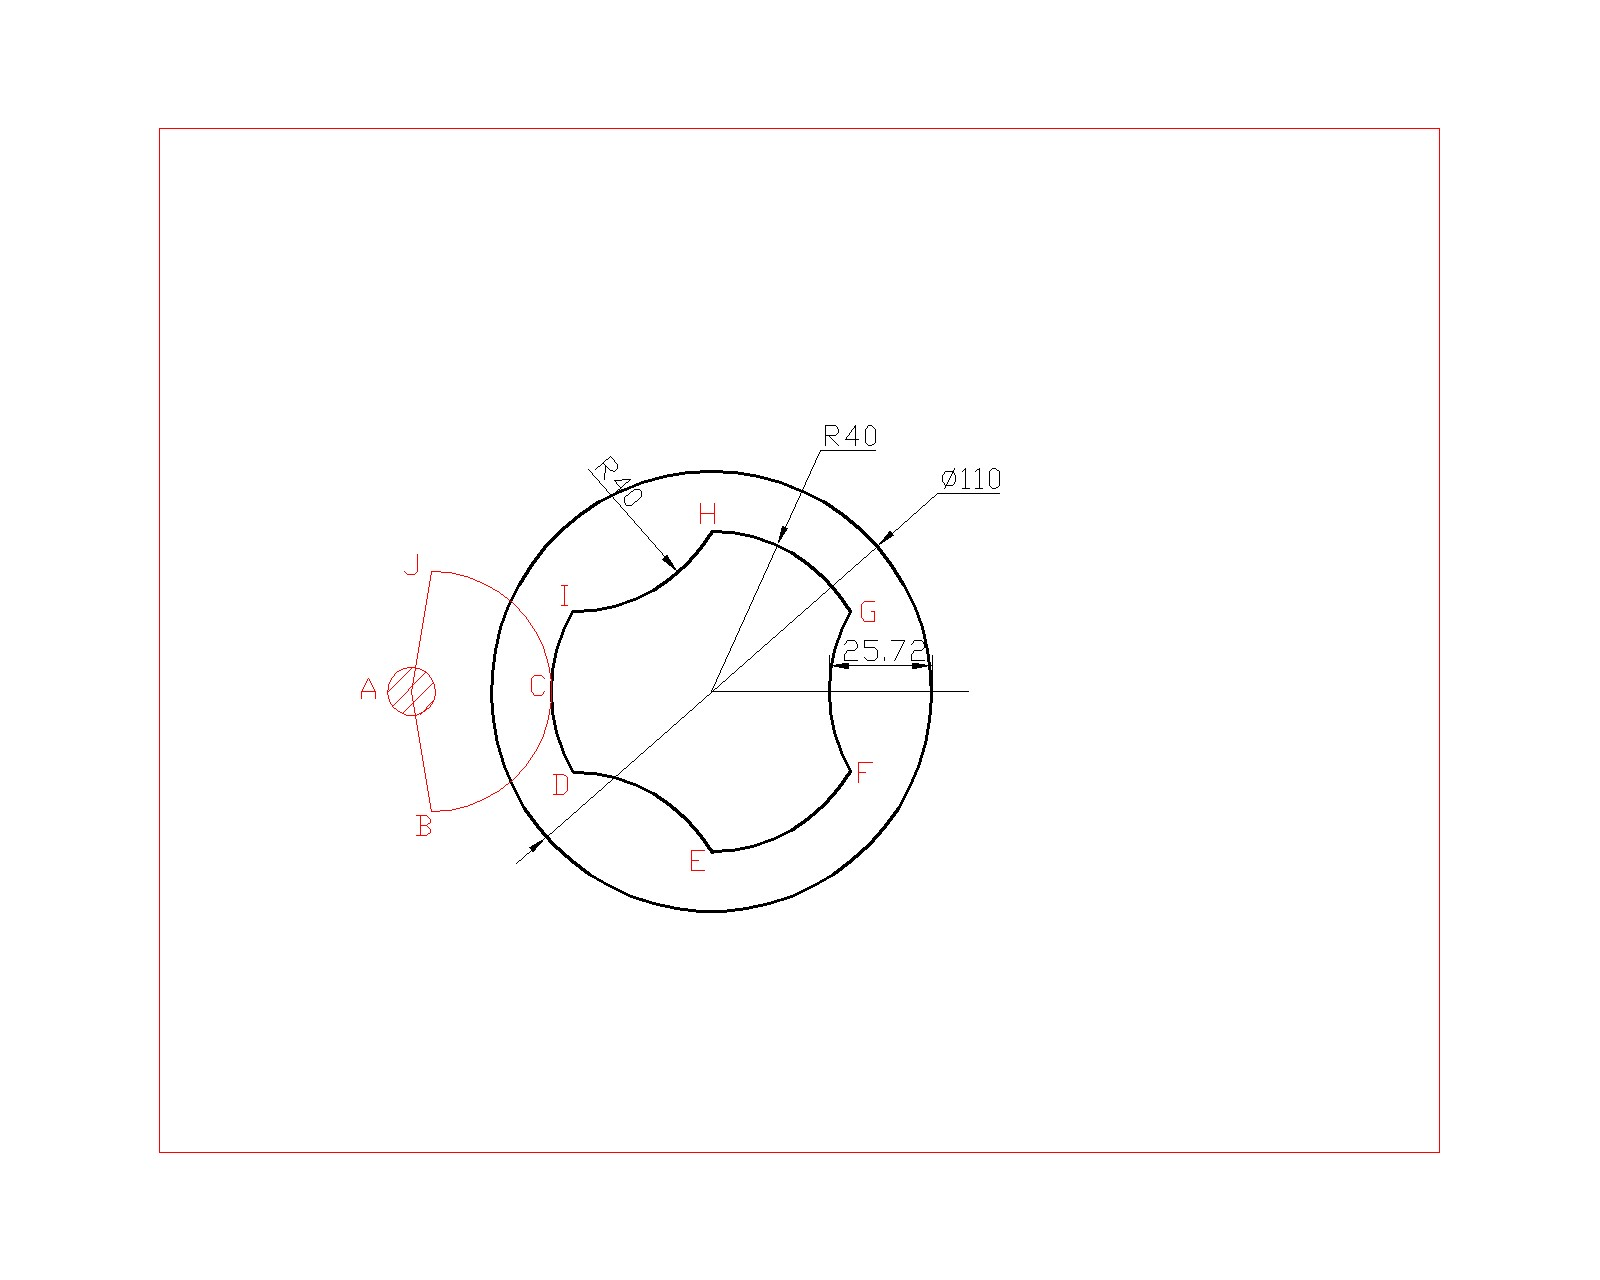
\includegraphics[width=0.8\linewidth,trim=280 250 430 280,clip]{data/image/8-2.jpg}
	\caption{刀补实例}
	\label{fig:9-1}
\end{figure}

1、计算最大残料值

以实际毛坯尺寸来计算  25.72

2、根据刀具直径确定粗加工刀补值

刀具半径+单边余量(0.2-0.6)

直径为12的立铣刀   6.5

3、根据刀具直径确定加工宽度

刀具直径的50\%-80\%   取10.

也可: (残料-粗加工刀补)/次数

4、刀补值的计算:

去残料刀补=粗加工刀补+加工宽度×次数

D2 16.5

D1 26.5

5、判断残料是否去完

最大刀补+刀具半径>最大残料  表示已去完

6、切入切出半径:

取R30

7、参考程序:
\begin{lstlisting}
O0001 (粗加工)
G54G17G40G49G90
M3S500
G1Z30.0F2000
X-75.0Y0
Z5.0
Z-5.0F200
G41X-70.Y-30.D1    (D1=26.5)
G3X-40.Y0R30.
G2X-34.64Y20.R40.
G3X0Y40.R40.
G2X34.64Y20.R40.
G3Y-20.R40.
G2X0Y-40.R40.
G3X-34.64Y-20.R40.
G2X-40.Y0R40.
G3X-70.Y30.R30.
G40G1X-75.Y0
G41X-70.Y-30.D1      (D2=16.5)
G3X-40.Y0R30.
G2X-34.64Y20.R40.
G3X0Y40.R40.
G2X34.64Y20.R40.
G3Y-20.R40.
G2X0Y-40.R40.
G3X-34.64Y-20.R40.
G2X-40.Y0R40.
G3X-70.Y30.R30.
G40G1X-75.Y0
G41X-70.Y-30.D1      (D3=6.5)
G3X-40.Y0R30.
G2X-34.64Y20.R40.
G3X0Y40.R40.
G2X34.64Y20.R40.
G3Y-20.R40.
G2X0Y-40.R40.
G3X-34.64Y-20.R40.
G2X-40.Y0R40.
G3X-70.Y30.R30.
G40G1X-75.Y0
M5
M30
\end{lstlisting}
精加工程序另写

\subsection{课堂小结}
\begin{enumerate}[1、]
	\item 去残料刀补的计算;
	\item 程序的编写
	
\end{enumerate}

\vfill
\subsection{布置作业}
\begin{enumerate}[1、]
	\item 写出上面的程序。
\item 习题集。 
\end{enumerate}
\vfill